\documentclass[
	a4paper,
	landscape,
	%twoside,
	10pt,
	article
]{article}
\usepackage[
	a4paper,
	landscape,
	twocolumn,
	left=0.8cm,
	right=0.3cm,
% Weird top and bottom margins because of fancyhdr package
	top=1.8cm,
	bottom=-0.3cm,
	columnsep=1cm,
% Set margins on even and odd pages equal
	hmarginratio=1:1,
	asymmetric
]{geometry}
\usepackage[english]{babel}
\usepackage[utf8]{inputenc}
\usepackage{textcomp}
\usepackage{amsmath}
\usepackage{amsfonts}
\usepackage{graphicx}
\usepackage{float}
\usepackage{listings}
\usepackage{color}
\usepackage[colorinlistoftodos]{todonotes}
\usepackage[compact]{titlesec}		% shrink section whitespace
\usepackage{ifthen}
\usepackage{nicefrac}
\usepackage{hyperref}

%*************** Layout ***************
\setlength{\columnseprule}{0.2pt}
\newcommand{\latexcolumnseprulecolor}{\color{red}}
\titlespacing{\section}{0pt}{0pt}{0pt}
\sloppy

% A red divider in the middle of the page
\usepackage{etoolbox}
\makeatletter
\patchcmd\@outputdblcol{% find
	\normalcolor\vrule
}{% and replace by
	\latexcolumnseprulecolor\vrule
}{% success
}{% failure
	\@latex@warning{Patching \string\@outputdblcol\space failed}%
}
\makeatother


%*************** Title ***************

% all the \vspace are for reducing the vertical spacing
\title{
	\vspace{-4em}
	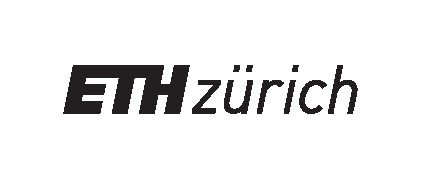
\includegraphics[scale=0.6]{./eth-logo.eps}\\
	\vspace{-1em}
	Team Code Reference
	\vspace{-0.7em}
}
%\author{ Timon Knigge, Ragnar Groot Koerkamp, \& Harry Smit }
\author{
	\Large \textbf{Team RaclETH}\\
}
\date{
	\vspace{-0.7em}
	SWERC 2018
	\vspace{-1.9em}
}


%*************** Table of Contents ***************
\usepackage[toc]{multitoc}			% multicolumn toc
\usepackage{tocloft}				% to reduce toc spacing
\renewcommand*{\multicolumntoc}{2}
% reduce section spacing in toc
\setlength{\cftbeforesecskip}{-1pt}
\setlength{\cftbeforesubsecskip}{-1.5pt}
% remove the toc title
\makeatletter
\renewcommand{\@cftmaketoctitle}{}
\makeatother


%*************** Headings ***************
\usepackage{fancyhdr}
\pagestyle{fancy}
\fancyhead{}
\fancyfoot{}
\setlength{\headsep}{0.4em}
\setlength{\footskip}{0em}

% one sided
\fancyhead[L]{\hspace{5em} ETH Z\"urich \phantom{-} \bfseries
Team RaclETH}
\fancyhead[R]{\thepage \hspace{0.5em}}
\fancyhead[C]{\leftmark}

%*************** Code highlighting ***************
\lstset{
	backgroundcolor=\color{white},
	tabsize=4,
	language=C++,
	basicstyle=\footnotesize\ttfamily,
	frame=lines,
	numbers=left,
	numberstyle=\tiny,
	numbersep=5pt,
	breaklines=true,
	keywordstyle=\color[rgb]{0, 0, 1},
	commentstyle=\color[rgb]{0, 0.5, 0},
	stringstyle=\color{red}
}


%*************** Section entries ***************
% \entry{name}{description}{snippet location}{complexity}{dependencies}
\newcommand{\entry}[3]{
	\subsection{#1}
	#2
	\ifthenelse{\equal{#3}{}}{}{\lstinputlisting[firstline=2]{#3}}
}
\newcommand{\pyentry}[3]{
	\subsection{#1}
	#2
	\ifthenelse{\equal{#3}{}}{}{\lstinputlisting[firstline=2,language=python]{#3}}
}
\newcommand{\otherentry}[3]{
	\subsection{#1}
	#2
	\lstinputlisting[language=]{#3}
}


%*************** Begin document ***************
\begin{document}


%*************** Reduce align spacing ***************
\setlength{\abovedisplayskip}{0pt}
\setlength{\belowdisplayskip}{0pt}
\setlength{\abovedisplayshortskip}{0pt}
\setlength{\belowdisplayshortskip}{0pt}

%*************** Titlepage ***************
{\let\newpage\relax\maketitle}
\tableofcontents
\textbf{Testsession}: Check if GNU builtins are available, as well as \texttt{\_\_int128}.
\thispagestyle{empty}
\newpage

%*************** Contents ***************


\subsection{Swiss keyboard}
\begin{figure}[H]
	\centering
	\includegraphics[scale=0.8]{ch.png}
\end{figure}

\subsection{Vim}
Turn off auto-tabbing by adding to the \texttt{.vimrc}: \texttt{filetype indent off}.

\subsection{Memory}
$10^5$ time $32$ bits is $0.4$ MegaBytes.
$10^6$ times $64$ bits is $8$ MB.
$10^6 \cdot \log 10^6$ times $64$ bits is $48$ MB.
In general, one megabyte is $8\cdot10^6$ bits. A \texttt{char},
\texttt{short}, \texttt{int}, \texttt{long long} is $8,16,32,64$
bits. A \texttt{float}, \texttt{double}, \texttt{long double} is
$32,64,80$ bits. Finally note $\log_2 10^{3k} \approx 10k$.

%\entry{C++ Header}{}{./snippets/header.h}
\subsection{C++}
Fast IO in C++: initialize with \texttt{ios::sync\_with\_stdio(false)}
and \texttt{cin.tie(nullptr)}. For debugging locally, it might help to
add \texttt{\#define \_GLIBCXX\_DEBUG}.
%\entry{Java Header}{}{./snippets/template.java}

\section{Datastructures}

\entry{Union Find}
{}
{./snippets/datastructures/unionfind.cpp}

\entry{Fenwick Tree}
{Can be generalized to arbitrary dimensions by duplicating loops.}
{./snippets/datastructures/fenwick.cpp}

\entry{Skew Heap}
{Meldable heap, all operations in $O(\log n)$ time.}
{./snippets/datastructures/skew-heap.cpp}

\entry{Segment Tree}{Works bottom up, so not suitable for lazy propagation.}
{./snippets/datastructures/segmenttree.cpp}

%\entry{Lazy Dynamic Segment Tree}
%{Here \texttt{T} is the data type and \texttt{U} the lazy update type.
%Implement all helper functions.}
%{./snippets/datastructures/segmenttree_dynamic.cpp}

\entry{Treap}{}{snippets/datastructures/treap.cpp}

\entry{Heavy-Light decomposition}{}
{./snippets/datastructures/heavylight.cpp}

\entry{Sequence}{This is essentially a treap, but it needs special
	functionality for the Euler Tour Tree}
{./snippets/datastructures/sequence.cpp}

\entry{Euler Tour Tree}{Maintain information about the trees using
	the underlying \texttt{seq} datastructure.}
{./snippets/datastructures/euler-tour-tree.cpp}

\entry{Suffix Array}{An $O(n \log n)$ implementation. Note that the resulting
	array maps values to their position in the suffix array, so invert if
	necessary.}
{./snippets/datastructures/suffixarray.cpp}

%\entry{Suffix Tree}{}{snippets/datastructures/suffix_tree.cpp}

\entry{Convex Hull Set}{}{./snippets/datastructures/convex-hull-set.cpp}

\entry{Pareto Front}{}{./snippets/datastructures/pareto-front.cpp}

\entry{GNU Built-in datastructures}
{These require \texttt{gnu} so check in test session.}
{./snippets/datastructures/builtin.cpp}

\section{Combinatorics}

\subsection{Formulae}
\subsubsection*{Permutations}
The number of derangements $D_n$, $n$-permutations without a fixed point,
satisfies $D_{n+1} = n(D_n + D_{n-1}) = (n+1)D_n + (-1)^{n+1}$. 
Stirling numbers of the first kind $S_1(n, k)$ count permutations on $n$ items
with $k$ cycles. $S_1(n, k) = S_1(n-1, k-1) + (n-1)S_1(n-1, k)$ with
$S_1(0, 0) = 1$. Note $\sum_{k=0}^n S_1(n, k)x^k = x(x+1)\dots(x+n-1)$.

Eulerian numbers $E(n, k)$ count the number of permutations on $n$ elments,
with exactly $k$ elements that are greater than their predecessor, i.e.
$k$ `ascents'. We have $E(n, k) = (n-k)E(n-1,k-1)+(k+1)E(n-1,k)$ with
$E(n, 0) = E(n, n-1)=1$.

\subsubsection*{Binomials and other partitionings}
We have $\binom{n}{k} = \binom{n-1}{k}+\binom{n-1}{k-1} =
	\prod_{i=1}^k \frac{n-i+1}{i}$. This last product may be computed
incrementally since any product of $k'$ consecutive values is divisibleby
$k'!$.

Basic identities: The hockeystick identity: $\sum_{k=r}^n \binom{k}{r}
	= \binom{n+1}{r+1}$
or $\sum_{k\leq n}\binom{r+k}{k} = \binom{r+n+1}{n}$.
Also $\sum_{k=0}^n \binom{k}{m} = \binom{n+1}{m+1}$.

For $n, m \geq 0$ and $p$ prime. Write $n, m$ in base $p$, i.e.
$n = n_k p^k + \dots + n_1 p + n_0$ and $m = m_k p^k + \dots m_1 p + m_0$. Then
by Lucas theorem we have $\binom{n}{m} \equiv \prod_{i=0}^k \binom{n_i}{m_i}
	\mod p$, with the convention that $n_i < m_i \implies \binom{n_i}{m_i} =0$.

\lstinputlisting[firstline=2]{snippets/combinatorics/binom.cpp}

We can put $n$ indistinguishable items into $k$ distinguishable bins in exactly
$\binom{n+k-1}{k-1}$ ways, or if we require the bins be non-empty, in
$\binom{n-1}{k-1}$ ways.

Stirling numbers of the second kind $S_2(n, k)$ count partitions of $n$
distinct elements into exactly $k$ non-empty groups.
$S_2(n, k) = S_2(n-1, k-1) + kS_2(n-1, k)$ with $S_2(n, 1) = S_2(n, n) = 1$ and
$$S_2(n, k) = \frac{1}{k!}\sum_{i=0}^k (-1)^{k-i}\binom{k}{i}i^n$$

Bell numbers $B_n$ count arbitrary partitions of $n$ distinct elements, i.e.
$B_n = \sum_k S_2(n, k)$.

\subsubsection*{Catalan numbers}
Catalan numbers $C_n$ satisfy $C_n = \frac{1}{2n+1}\binom{2n}{n}$ as well
as $C_0 = 1, C_{n+1} = \sum_i C_i C_{n-i}$. These count, among other things:
	Valid parenthesis sequences of length $2n$.
	Sub-diagonal monotone paths from $(0, 0)$ to $(n, n)$ in the
		$n\times n$ grid.
	Complete binary trees (i.e. no vertices with exactly $1$ child)
		with $n+1$ leaves.
	Triangulations of a convex polygon with $n+2$ sides.
	Stack-sortable permutations of size $n$.

\subsubsection*{Trees}
There are $n^{n-2}$ labeled unrooted (cq. $n^{n-1}$ rooted) trees on $n$
vertices. A bijection between a tree and it's Pr\"ufer sequence
$(a_1, a_2, \dots, a_{n-2})$is given by:
\begin{enumerate}
	\item[$\leftarrow$] Given the Pr\"ufer sequence $(a_j)_{j=1}^{n-2}$,
		let $d_i$ be $1$ plus the
		number of occurences of $i$ in $a$. Now for each $a_j$ for $j=1\dots$,
		find the lowest
		numbered node $k$ with degree $1$ and add $\{a_j, k\}$, and decrement
		the degrees $d_{a_j}, d_k$. At the end two degree $1$ nodes remain,
		connect them.
	\item[$\rightarrow$] Iterate, at step $i=1,\dots,n-2$ remove the leaf with the
		smallest label and set the $i^{th}$ element of $a$ to be its
		neighbour. 
\end{enumerate}

\subsection{Burnside's lemma}
Given a group $G$ acting on a set $X$, the number of elements in $X$ up to
symmetry is $$\frac{1}{|G|}\sum_{g\in G} |X^g|$$ with $X^g$ the elements of
$X$ invariant under $g$. For example, if $f(n)$ counts ``configurations''
of some sort of length $n$, and we want to count them up to rotational symmetry
using $G = \mathbb{Z}/n\mathbb{Z}$, then

$$g(n) = \frac{1}{n} \sum_{k=0}^{n-1} f(\gcd(n, k))
	= \frac{1}{n}\sum_{k \| n} f(k) \phi(n / k)$$

I.e. for coloring with $c$ colors we have $f(k) = k^c$.

Relatedly, in P\'olya's enumeration theorem we imagine $X$ as a set of $n$
beads with $G$ permuting the beads (e.g. a necklace, with $G$ all rotations and
reflections of the $n$-cycle, i.e. the dihedral group $D_n$).
Suppose further that we had $Y$ colors, then
the number of $G$-invariant colorings $Y^X / G$ is counted by

$$\frac{1}{|G|}\sum_{g\in G} |Y|^{c(g)}$$

with $c(g)$ counting the number of cycles of $g$ when viewed as a permutation
of $X$. We can generalize this to a weighted version: if the color $i$ can
occur exactly $r_i$ times, then this is counted by the coefficient of
$t_1^{r_1}\dots t_n^{r_n}$ in the polynomial
$$Z(t_1,\dots,t_n) = \frac{1}{|G|}\sum_{g\in G} \prod_{m\geq 1}
	(t_1^m+\dots+t_n^m)^{c_m(g)}$$
where $c_m(g)$ counts the number of length $m$ cycles in $g$ acting as a
permutation on $X$. Note we get the original formula by setting all $t_i=1$.
Here $Z$ is the cycle index. Note: you can cleverly deal with even/odd sizes
by setting some $t_i$ to $-1$.


\subsection{Inclusion-Exclusion}

For appropriate $f$ compute $\sum_{S\subseteq T} (-1)^{|T\setminus S|} f(S)$,
or if only the size of $S$ matters, $\sum_{s=0}^n (-1)^{n-s} \binom{n}{s}f(s)$.
In some contexts we might use Stirling numbers, not binomial coefficients!

Some useful applications:
\begin{enumerate}
	\item[] \textbf{Graph coloring} Let $I(S)$ count the number
		of independent sets
		contained in $S \subseteq V$ ($I(\emptyset) = 1$,
		$I(S) = I(S\setminus v) + I(S\setminus N(v))$). Let
		$c_k = \sum_{S\subseteq V} (-1)^{|V\setminus S|} I(S)$. Then $V$
		is $k$-colorable iff $v > 0$. Thus we can compute the chromatic
		number of a graph in $O^*(2^n)$ time.
\end{enumerate}

\entry{Subset enumeration}
{Note: for sum over subsets use FSC.}
{./snippets/utils/bitmasking.cpp}

Some related gnu built-in functions that might be useful. Note that all of
these take \textit{unsigned} values!!
\begin{description}
	\item[\texttt{\_\_builtin\_popcount[ll](x)}] Counts the number of $1$s in
		{\tt x}.
	\item[\texttt{\_\_builtin\_ctz[ll](x)}] Counts the number of trailing $0$s
		in {\tt x}. In other words, the exponent of the largest power of $2$
		dividing {\tt x}.
	\item[\texttt{\_\_builtin\_clz[ll](x)}] Counts the number of leading $0$s
		in {\tt x}.
\end{description}

\entry{Fast Subset Convolution}
{Sets $a'(S) = \sum_{T\subseteq S} a(T)$ in $O(n2^n)$ time (rather than
$O(3^n)$ or even $O(4^n)$). Note that if you flip the \texttt{+=} to a
\texttt{-=} you get inclusion-exclusion for all subsets!}
{./snippets/combinatorics/fsc.cpp}

\subsection{Stable Marriage Algorithm}
Given $n$ men and $n$ women, with each man ranking each woman by preference,
and vice versa, (i.e., permutations),
we can find a stable marriage by applying this procedure:
\begin{itemize}
	\item Initialize all men $m$ and women $w$ to `free'.
	\item While there is a free man $m$ for whom there is some woman $w$ he
		has not proposed to, let $w$ be the first/most prefered such woman. Now
		$m$ proposes to $w$.
	\begin{itemize}
		\item If $w$ is free, then $(m, w)$ become engaged.
		\item If $w$ is engaged to $m'$ and $w$ prefers $m'$, nothing happens.
		\item If $w$ is engaged to $m'$ and $w$ prefers $m$, then $(m, w)$
			become engaged and $m'$ becomes free.
	\end{itemize}
\end{itemize}
Implement in $O(n^2)$ with the right bookkeeping. The resulting configuration
marries everyone, with no unstable marriages (where two unmarried people prefer
each other to their partners). When the number of men/women don't match add
dummy people noone prefers.

\entry{Bron-Kerbosch}
{Maximal clique enumeration, runs in about $O(3^{n/3})$ time (or
	$O(\#cliques)$).}
{./snippets/graphs/bronkerbosch.cpp}

\entry{$2$-SAT}{}
{./snippets/combinatorics/2-sat.cpp}

\entry{Simplex Algorithm}
{Maximize $c^tx$ subject to $Ax\leq b$ and $x\geq 0$. With
$A[m\times n], b[m], c[n], x[n]$. Solution in $x$.
The dual problem is to maximize $b^tx$ subject to $A^tx\geq c$.
Strong duality says the optima coincide.}
{./snippets/combinatorics/simplex.cpp}

\section{Mathematics}

\entry{Elementary Number Theory}{}{snippets/math/elementary-nt.cpp}
\entry{Chinese Remainder Theorem}{}{snippets/math/crt.cpp}
\entry{Tonelli-Shanks}{}{snippets/math/tonelli-shanks.cpp}
\entry{Euler-Phi function}{
For $n>0$, $\phi(n)$ counts all numbers in $\{1, \dots, n-1\}$ coprime to $n$.
Note for $n = {p_1}^{k_1}\dots p_m^{k_m}$ we have
$$\phi(n) = n \prod_i \frac{p_i-1}{p_i} = n\prod_i \big(1-\frac{1}{p_i}\big)$$
Also $\sum_{d\|n} \phi(d) = n$. Finally for $a$ and $n$ relatively prime,
$a^{\phi(n)} \equiv 1 \mod n$.
}{snippets/math/phi.cpp}

\entry{Floor sums}{All in $O(\log n)$ time.}{snippets/math/floor-sums.cpp}

\pyentry{Continued Fractions}{
Continued fractions are typically written as:
$$
	[a_0; a_1, a_2, \dots] \leftrightarrow a_0 + \cfrac{1}{a_1 + \cfrac{1}{a_2 + \tfrac{1}{\dots}}}
$$
Particularly well-known is $e \leftrightarrow [2;1,2,1,1,4,1,1,6,1,1,8,\dots]$ and $\phi \leftrightarrow
	[1;1,1,\dots]$. The continued fraction representation of a number $r \in \mathbb{R}$ is finite if
	and only if $r \in \mathbb{Q}$. Real numbers with a periodic continued fraction are exactly the
	quadratic irrationals (roots of irreducible quadratics in $\mathbb{Q}[X]$, i.e. $\tfrac{a+b\sqrt{c}}{d}$
	with $c$ square free).

The convergents of a continued fraction $r \leftrightarrow [a_0; a_1, a_2, \dots]$ are given as
	$\tfrac{h_0}{k_0} = \tfrac{a_0}{1}$, $\tfrac{h_1}{k_1} = \tfrac{a_1 a_0 + 1}{a_1}$
	and $\tfrac{h_n}{k_n} = \tfrac{a_n h_{n-1} + h_{n-2}}{a_n k_{n-1} + k_{n-2}}$. This sequences has the
	following useful properties:

	$$[a_0; a_1, \dots, a_{n-1}, z] = \frac{z h_{n-1} + h_{n-2}}{z k_{n-1} + k_{n-2}}$$
	$$\gcd(h_n, k_n) = 1$$
	
	Also, the even convergents continually increase, whereas the odd convergents always decrease. Most
	importantly, these convergents give, in some sense, an `optimal' approximation to $r$, that is,
	for any $\tfrac{h_n}{k_n}$ there exists no closer rational to $r$ with smaller numerator
	or denominator.

	Finally (Pell's equation), for positive integers $p, q$ and non-square $n$, it holds that
	$p^2 - nq^2 = \pm 1$ if and only if $\tfrac{p}{q}$ is a convergent of $\sqrt{n}$. Here, the
	following relation is useful for computing convergents of $\sqrt{D}$ where $D = \tfrac{p}{q}$:
	take $a_0 = \lfloor \sqrt{D} \rfloor, b_1 = a_0, c_1 = D - a_0^2$, and follow

	$$a_{n-1} = \lfloor \tfrac{a_0 + b_{n-1}}{c_{n-1}}\rfloor, b_n = a_{n-1}c_{n-1} - b_{n-1},
		c_n = \tfrac{D-b_n^2}{c_{n-1}}$$
	Here $b_n$ and $c_n$ remain bounded by $2\sqrt{D}$.
	Maintain a cache to find the eventual period. The length of the period is bounded by $pq$, though
	usually it is much smaller. In fact, for $D \in \mathbb{Z}$ the period is $O(\sqrt{D}\log D)$.
	Additionally, the period will repeat from the second term,
	simplifying caching.
}{snippets/math/continued-fraction.py}

\subsection{Enumerating $\mathbb{Q}$}
For the \textbf{Stern-Brocot tree}, initially take the two `fractions'
$\tfrac{0}{1}$ and $\tfrac{1}{0}$. For any two fractions $\tfrac{a}{b}$ and
$\tfrac{c}{d}$ define their mediant as $\tfrac{a+c}{b+d}$. We can iterate this
process on every new layer of the tree, so the first value (the root) will be
$\tfrac{0+1}{1+0} = \tfrac{1}{1}$, then $\tfrac{0+1}{1+1} = \tfrac{1}{2}$ and
$\tfrac{1+1}{1+0} = \tfrac{2}{1}$, etc. This tree satisfies:
\begin{enumerate}
	\item All rationals are enumerated in their lowest terms, exactly once.
	\item If $\tfrac{a}{b}$ is a direct ancestor of $\tfrac{c}{d}$ then
		$ad - bc = \pm 1$.
\end{enumerate}

The \textbf{Farey sequence} of order $n$ is the sorted sequence of rationals in
$[0, 1]$ in lowest terms whose denominators do not exceed $n$, e.g.
$F_4 = \{0/1, 1/4, 1/3, 1/2, 2/3, 3/4, 1/1\}$. Note that
$|F_n| = |F_{n-1}| + \phi(n) = 1 + \sum_{k=1}^n \phi(k)$.
We can generate the Farey sequence in a manner
similar to the Stern-Brocot tree, inserting $\tfrac{a+c}{b+d}$ between
$\tfrac{a}{b}$ and $\tfrac{c}{d}$ when $c+d \leq n$.

\entry{Primes}{Note that sieving into a bitset might be more space
efficient.
\begin{table}[h]
	\begin{tabular}{|l|ccccc|}
	\hline
	$\leq N$ & $10^3$ & $10^6$ & $10^9$ & $10^{12}$ & $10^{18}$ \\
	\hline
	$m$	& $840$ & $720720$ & $735134400$ & $963761198400$ & $897612484786617600$ \\
	\hline
	$d(m)$ & $32$ & $240$ & $1344$ & $6270$ & $103680$ \\
	\hline
	\end{tabular}
	\centering
	\caption{Maximizers of $d(n)$ upto some bound $N$.}
\end{table}
}{snippets/math/primes.cpp}

\entry{Lucy's algorithm}{Modified Meissel-Lehmer algorithm for summing
complete multiplicative functions over the primes up to $n$ 
in $O(n^{3/4})$ time. Example \texttt{f} and \texttt{F} compute the sum
of squares.}{snippets/math/lucy.cpp}

\entry{Miller-Rabin}{}{snippets/math/miller_rabin.cpp}
\entry{Pollard-$\rho$}{}{snippets/math/pollard-rho.cpp}

\entry{Finite Field}{For usage with FFT.}{snippets/math/field.cpp}
\entry{Complex Field}{For usage with FFT.}{snippets/math/complex.cpp}
\entry{Fast Fourier Transform}{Use Finite Field for NTT. For the complex FFT,
\texttt{double} is noticably faster ($>2$x) than \texttt{long double}. Use
high precision FFT when worried about precision.}
{snippets/math/fft.cpp}

\subsection{Fast Walsh-Hadamard Tr.}
To compute the xor convolution of $(a_i)_{i=0}^{2^k-1}$ and
	$(b_j)_{j=0}^{2^k-1}$, given as $c_k = \sum_{i \oplus j = k} a_i b_j$, use
the Hadamard matrix $[[1,1], [1,-1]]$ inside of the inner loop of the FFT. In
practice, this just means using $\omega = 1$. In particular, there is no need
to compute roots and this transform works in any finite field
$\mathbb{Z} /p\mathbb{Z}$.

\entry{High-Precision Convolution}{A \texttt{double} is precise for all integers
upto $2^{53}\approx 9e15$. This version breaks up the FFT in lower and upper
15 bits.}{snippets/math/high-prec-convolution.cpp}

\entry{Polynomial Arithmetic}{Power series inversion and polynomial division
each in $O(n \log n)$ time.}{./snippets/math/poly.cpp}
 Some other useful operations:
\begin{description}
	\item[$\sqrt{P(x)}$] Like Hensel lifting for the inverse, start with
		a solution $\mod x$. Then if $S_n(x)^2 = P(x) \mod x^n$, we have
		$$S_{2n}(x) = \frac{1}{2}(S_n(x) + F(x)S_n(x)^{-1}) \mod x^{2n}$$
\end{description}

\entry{Linear Recurrence Solver}{Given a linear recurrence of the form
$$a_n = \sum_{i=0}^{k-1} c_i a_{n-i-1}$$
this code computes $a_n$ in $O(k \log k \log n)$ time. However, in practice
the constant factor is quite large. On codeforces it runs in about $1200$ms
for $k=3000$ and $n=10^{18}$. Caching inverses for each input \texttt{n}
gives about $800ms$.}{snippets/math/lin-rec.cpp}

\entry{Matrix Solver}{}{snippets/math/matrix_solve.cpp}

\entry{Matrix Exponentiation}{Note: swapping the last two loops of the
multiplication helps with speed (due to cache).}
{snippets/math/matrix_exp.cpp}

\subsection{Game theory}
A game can be reduced to Nim if it is a finite impartial game, then for any
state $x$, $g(x) = \inf (\mathbb{N}_0 - \{g(y) : y \in F(x) \})$. Nim and
its variants include:
\begin{description}
	\item[Nim] Let $X = \bigoplus_{i=1}^n x_i$, then $(x_i)_{i=1}^n$ is a
		winning position iff $X\neq 0$. Find a move by picking $k$ such
		that $x_k > x_k \oplus X$.
    \item[Misère Nim] Regular Nim, except that the last player to move
		\textit{loses}. Play regular Nim until there is only one pile of size
		larger than $1$, reduce it to $0$ or $1$ such that there is an odd
		number of piles.
    \item[Moore's Nim$_k$] The player may remove from at most $k$ piles
		(Nim $=$ Nim$_1$). Expand the piles in base $2$, do a carry-less
		addition in base $k+1$ (i.e. the number of ones in each column
		should be divisible by $k+1$).
    \item[Lasker's Nim] Players may alternatively split a pile into two new
		non-empty piles. $g(4k+1) = 4k+1$, $g(4k+2) = 4k+2$, $g(4k+3) = 4k+4$,
		$g(4k+4) = 4k+3$ ($k\geq 0$).
    \item[Hackenbush on trees] A tree with stalks $(x_i)_{i=1}^n$ may be
		replaced with a single stalk with length $\bigoplus_{i=1}^n x_i$.
\end{description}
For others, bruteforce $g$ for small $x$ and try to spot a pattern. And
a useful identity: $\bigoplus_{x=0}^{a - 1} x = \{0, a - 1, 1, a\}[a \% 4]$.

\section{Graph Algorithms}

\entry{Tarjan's Algorithm}{}
{./snippets/graphs/tarjan.cpp}

\entry{Biconnected Components}{}
{./snippets/graphs/biconnected_component.cpp}

\entry{MDST}{Minimum directed spanning tree rooted at some $r$. Runs in $O(E \log V)$. About $3$s for a
complete graph on $n=2500$ vertices on Kattis.}
{./snippets/graphs/arborescence.cpp}

\entry{Eulerian paths and tours}
{In an \textit{undirected graph}, an \textit{Eulerian Circuit} exists iff
all vertices have even degree, and all vertices of nonzero degree
belong to a single connected component. In an \textit{undirected graph},
an \textit{Eulerian Trail} exists iff at most two vertices have
odd degree, and all vertices of nonzero degree belong to a single
connected component. In a \textit{directed graph}, an \textit{Eulerian Circuit}
exists iff every vertex has equal indegree and outdegree, and all
vertices of nonzero degree belong to a single strongly connected component.
In a \textit{directed graph}, an \textit{Eulerian Trail} exists iff
at most one vertex has $d_{out} - d_{in} = 1$, at most one vertex has
$d_{in} - d_{out} = 1$, every other vertex has equal indegree and
outdegree, and all vertices of nonzero degree belong to a single
connected component \textit{in the underlying undirected graph}.}
{./snippets/graphs/euleriancircuits.cpp}

\entry{Bellmann-Ford}{$O(VE)$}{./snippets/graphs/bellmannford.cpp}

\subsection{Johnson's reweighting}
For computing all pairs shortest paths in sparse graphs with negative weights.
Apply Bellman-Ford to the graph with \texttt{d[u] = 0} (as if an extra
vertex with zero weight edges were added), then reweight edges to
$w_{uv} + h_u - h_v$, then use Dijkstra from every vertex.
The result is $O(VE + (V+E)(\log E))$.

\subsection{Tree isomorphisms}
For a rooted tree isomorphism, from the lowest level to the highest, compute
a hash for each subtree based on the ordered or unordered set of hashes of
the children. This can be implemented deterministically and fast using radix
sorts, but this takes a lot of code - use strong hash functions instead. An
example of a good hash function is to pick $s_d \in \mathbb{F}_p$ uniformly
at random for each depth $d$ and hash a vertex $v$ at depth $d$ to
$h_v = s_d + \prod_{u \text{ child of } v} h_u$.

For an unrooted tree isomorphism, try finding a rooted tree isomorphism between
all pairs of centroids.

\subsection{Relevant Theorems}
\begin{description}
\item[Kirchhoff's Theorem]
Given an undirected graph $G$ on $n$ vertices, let $D$ be the $n\times n$
matrix with all degrees on the diagonal, and $A$ the $n\times n$ incidence
matrix of $G$. Let $M$ be any minor (remove one row and one column) of $D-A$.
Then the number of spanning trees of $G$ is $|\det M|$.
\item[Acyclicity]
A directed graph is acyclic if and only a depth-first search yields no back
edges.
\end{description}

\section{Flows and cuts}
\entry{Flow Graph}
{Datastructure used by all flow algorithms}
{./snippets/flowalgorithms/flowgraph.cpp}

\entry{Dinic Algorithm}
{Runs in $O(V^2 E)$, or $O(VE \log U)$ after introducing scaling. On unit
capacity networks it runs in $O(\min\{V^{2/3}, E^{1/2}\}E)$ time. On networks
where every vertex has either a single incoming edge that also has unit capacity,
or a single outgoing edge that also has unit capacity, it runs in $O(E\sqrt{V})$.}
{./snippets/flowalgorithms/dinic.cpp}

%\entry{Minimum Cut Inference}{}
%{./snippets/flowalgorithms/infermincut.cpp}

\entry{Minimum Cost Flow}
{Cannot handle negative cycles}
{./snippets/flowalgorithms/mincostflow.cpp}

\entry{Minimum Cost Circulation}
{Fast in practice, can easily do min cost matching upto $n=1000$.}
{snippets/flowalgorithms/min-cost-circulation.cpp}

\subsection{Relevant Constructions}
\begin{description}
	\item[Circulation] Add a supersource S and supersink T. For an arc
		$(x, y)$ with lowerbound $l$ and upperbound $u$, set its new
		capacity to $u-l$, and add arcs $(S, y)$ and $(x, T)$ with capacity
		$l$. Then find a flow from $S$ to $T$. This corresponds to a
		circulation if the flow equals $\sum_{(x, y)} l$. Note: This approach
		can often be sped up significantly by merging double edges.
	\item[Tutte matrix] For a graph $G = (V, E)$, its Tutte matrix $T$ is
		defined as $T_{ij}$ equal to $0$ if $\{i, j\}\not\in E$, $x_{ij}$
		if $i < j$ or $-x_{ji}$ if $i > j$. The rank of $T$ is twice the size
		of the maximum matching in $G$. To compute: assign $x_{ij}$ randomly
		in $\mathbb{F}_p$ and compute the rank for some number of iterations $k$.
		Take the maximum over all runs, for a total runtime of $O(kn^3)$. Each
		iteration has a failure probability of at most $n / p$. Also
		relevant for reconstruction is the Rabin-Vazirani lemma: if $G$ has a
		perfect matching then $G - \{v_i, v_j\}$ has a perfect matching if
		$(T^{-1})_{ij} \neq 0$ where $T$ is the Tutte matrix of $G$.
	\item[Project selection] A very non-trivial application of flow is the
		project selection problem, where we have a set of projects $P$, and
		each project $i\in P$ has an associated revenue $p_i$ (which can be
		positive or negative). There are dependencies between the projects,
		given by some acylic graph $G=(P, A)$ (cyclic dependencies can just
		be collapsed into a single vertex). The goal is of course to select 
		some set of projects $S \subseteq P$ so as to maximize
		profit while satisfying the dependencies.

		To solve, build a flow graph $G'$ with $(s, i)$ with capacity $p_i$
		if $p_i > 0$, or $(i, t)$ with capacity $-p_i$ if $p_i<0$. Furthermore
		add infinite capacity edges to $G'$ for the edges of $G$. Let
		$C = \sum_{p_i > 0} p_i$, then we claim that for any cut $(A', B')$,
		the set $A = A\setminus\{s\}$ is a set of projects that satisfies
		$c(A', B') = C - \sum_{i\in A} p_i$. Therefore the minimum $(s, t)$-cut
		in $G'$ solves the problem.
\end{description}

\subsection{Relevant Theorems}
\begin{description}
	\item[Min-Cut Max-Flow] The minimum cut separating $s$ and $t$ equals the
		maximum flow between $s$ and $t$.
	\item[K\"onigs Theorem] There is a bijection between the maximum matchings
		in a bipartite graph and the minimal vertex covers. To find the cover:
		find a maximum matching and run minimum cut inference. Then pick all
		vertices that are on the `wrong' side. Also note the complement of a
		minimum vertex cover is a maximum independent set.
	\item[Hall's Marriage Theorem] For a bipartite graph $(L \cup R, E)$, a
		matching saturating $L$ exists iff $\forall L' \subseteq L$ we have
		$|L'| \leq |N(L')|$ where $N(L')$ is the neighbour set of $L'$.
	\item[Dilworth's Theorem] The minimum number of disjoint chains into which
		a partial ordering $S$ can be decomposed equals the length of
		the longest antichain of
		$S$. Compute by defining a bipartite graph with $l_x$ and $r_x$ for
		each $x \in S$, and add $(l_x, r_y)$ if $x < y$. For
		a maximum matching of size $m$ the number of disjoint chains is then
		$|S|-m$. To find the actual antichain, find the minimal vertex cover
		and take all $x$ with neither $l_x$ nor $r_x$ in the cover.
	\item[Mirsky's Theorem] Dual theorem to the above, for the smallest
		decomposition into antichains and the longest chain. Easily computable
		using dynamic programming.
\end{description}

\subsection{Karger's Algorithm}
To find a minimum cut in a graph, repeatedly contract a random edge until there
are only two components left. One easy way to implement this is to randomly
give each edge a weight, and then run Kruskal's algorithm until only two
components are left. To find the cut with high probability, repeat the algorithm
$\binom{n}{2}\log{n}$ times for a failure probability of $\frac{1}{n}$. The
total running time is then $O(n^2 m \log{n})$.

\entry{Gomory-Hu Tree}{Does $V-1$ minimum cut computations. Useful: taking the
	$k-1$ lightest edges in the tree gives a $2-2/k$ approximation to the
	minimum $k$-cut problem}{./snippets/flowalgorithms/gomory-hu-tree.cpp}

\section{Dynamic Programming}

\entry{LIS}
{For the actual sequence, store parent pointers. Note that longest common
subsequence can be reduced to LIS with unique elements.}
{./snippets/dp/lis.cpp}

\entry{All Nearest Smaller Values}{}{./snippets/dp/ansv.cpp}

\subsection{DP Optimizations}
\begin{enumerate}
	\item[CH] Recurrences are generally of the form
		$dp_i = dp_j \cdot a_i + b_j$ or equivalent. Insert all lines as
		functions of $a_i$ into the convex hull set (see datastructures) to
		query in logarithmic time.
	\item[DC] Recurrences are generally of the form
		$dp_{k,i} = \max_{j<i} f(dp_{k-1,j}, i, j, k)$. If the $\arg\max$ is
		monotonic in $i$, do divide and conquer by first finding the answer
		for $i = \frac{n}{2}$, and then recursing for larger and smaller $i$.
	\item[Knuth] Recurrences are generally of form similar to
		$$dp_{i,j} = min_{i\leq k<j} \big(f(i, j) + dp_{i,k} + dp_{k+1,j}\big)$$
		Let $a_{i,j}$ be the $\text{argmin}$ for $dp_{i, j}$, then if
		$a_{i,j-1} \leq a_{i, j} \leq a_{i+1,j}$, for a fixed $len > 0$ the
		ranges we have to scan for all $dp_{i, i+len}$ are (almost) disjoint,
		and we can solve the recurrence in $O(n^2)$ time.

		A sufficient condition for applicability on $f$ is, for
		$i\leq j\leq k\leq l$, monotonicity: $f(j,k) \leq f(i, l)$, and
		the quadrangle inequality: $f(i,k)+f(j,l)\leq f(i,l)+f(j,k)$.
\end{enumerate}

\section{Geometry}
\textbf{\color{red} Use 64-bit integer arithmetic whenever possible.}

\subsection{Formulae I}
To \textbf{intersect two lines}, assume by equations of the form
$ax + by = e$. For a line going through points $(x_1, y_1)$ and
$(x_2, y_2)$, note that $\vec{n} = (y_1 - y_2, x_2 - x_1)$ is a normal vector,
so the line equation is given by $\vec{n}\cdot\vec{p}
	 = \vec{n} \cdot (x_1, y_1)$ for
$\vec{p} \in \mathbb{R}^2$. Note: normalizing $\vec{n}$ might be necessary due
to input sizes, but this does result in a loss of precision. Then:
$$\begin{aligned}ax+by=e\\cx+dy=f\end{aligned}
\,\to\,
\begin{aligned}x=\dfrac{ed-bf}{ad-bc}\\y=\dfrac{af-ec}{ad-bc}\end{aligned}$$

This equation is undefined precisely when $ad-bc = 0$, i.e. the given lines
coincide ($e=f$) or are parellel ($e \neq f$). For segment-segment
intersections, just check that $(x, y)$ is in the bounding box of the two
segments.
For a general equation of the form $Ax = b$, we have $x_i = \det A_i / \det A$
with $A_i$ equal to $A$ with the $i^{th}$ column replaced by $b$.

When only \textbf{deciding whether two segments intersect}, there is no need
to compute the intersection point, use determinants instead (or rather,
the derived \texttt{ccw} function). Specifically, the sequence $\vec{a}
	\to \vec{b} \to \vec{c}$ goes counterclockwise iff
$(\vec{b}-\vec{a})\times(\vec{c}-\vec{a})$ is positive, and clockwise if it
is negative. Colinearity if and only if the determinant is $0$. For example:

\lstinputlisting[firstline=2]{snippets/geometry/segseg.cpp}

In \texttt{C++}, the angle between $(x_1, y_1)$ and $(x_2, y_2)$ is
\texttt{atan2(y1-y2, x1-x2)}. Note that it returns values in
$(-\pi, \pi]$. In general though, when sorting by angle, try to use
determinants to avoid precision errors.

The \textbf{projection} of $\vec{u}$ onto $\vec{v}$ is
$\lambda\vec{v}$ for $\lambda = \frac{\vec{u}\cdot\vec{v}}{|\vec{v}|^2}$.
When projecting on a segment, truncate $\lambda$ to $[0, 1]$.

The \textbf{reflection} of $\vec{q}$ through the line $\vec{p_1}\to\vec{p_2}$
is $2\vec{q'} - \vec{q}$ where $\vec{q'}$ is the projection of $\vec{q}$ onto
the line (see above).

To do a \textbf{line-circle intersection} project the center of the circle onto
the line, and move left/right over the line using Pythagoras theorem.

The line intersecting two three-dimensional planes can be found by taking the
cross product of their normal vectors. The three dimensional cross product is
given as:
$$\begin{aligned}
	\begin{bmatrix}
		x_1 \\ y_1 \\ z_1
	\end{bmatrix}
	&\times
	\begin{bmatrix}
		x_2 \\ y_2 \\ z_2
	\end{bmatrix}
	=
	\begin{bmatrix}
		y_1 z_2 - y_2 z_1 \\
		z_1 x_2 - z_2 x_1 \\
		x_1 y_2 - x_2 y_1
	\end{bmatrix}
\end{aligned}$$
Given $\vec{p}, \vec{q}, \vec{r} \in \mathbb{R}^3$, the associated plane
is defined by $\vec{x} \cdot \vec{n} = \vec{r}\cdot\vec{n}$ for
$\vec{n} =(\vec{p}-\vec{r})\times(\vec{q}-\vec{r})$.

\entry{2D Geometry Utilities}{}{snippets/geometry/essentials.cpp}

\subsection{Formulae II}
\begin{equation*}
	[ABC]
	= rs
	= \frac 12 ab\sin\gamma
	= \frac{abc}{4R}
	= \sqrt{s(s-a)(s-b)(s-c)}
	= \frac 12\left| (B-A, C-A)^T \right|
\end{equation*}

\begin{align*}
	s &= \frac {a+b+c}2 & 2R &=\frac{a}{\sin \alpha}\\
	\textrm{cosine rule:}&&  c^2 &= a^2 + b^2 - 2ab\cos \gamma\\
	\textrm{Euler:}&&  1 + CC &= V - E + F\\
	\textrm{Pick:}&& \textrm{Area} &= \textrm{interior points}
	+ \frac{\textrm{boundary points}}2 - 1\\
	p\cdot q &= |p||q|\cos(\theta) & |p\times q| &= |p||q|\sin(\theta)\\
\end{align*}

Given a non-self-intersecting closed polygon on $n$ vertices, given as $(x_i, y_i)$, its centroid $(C_x, C_y)$ is given as:

\begin{align*}
	C_x &= \frac{1}{6A} \sum_{i = 0}^{n - 1} (x_i + x_{i+1}) (x_i y_{i+1} - x_{i+1} y_i), &
	C_y &= \frac{1}{6A} \sum_{i = 0}^{n - 1} (y_i + y_{i+1}) (x_i y_{i+1} - x_{i+1} y_i)
\end{align*}

\begin{equation*}
	A = \frac{1}{2} \sum_{i = 0}^{n - 1} (x_i y_{i+1} - x_{i+1} y_i) = \textrm{polygon area}
\end{equation*}

\entry{Planar Rotation}{}{snippets/geometry/planar-rotation.cpp}

\entry{Convex Hull}{}
{snippets/geometry/convexhull.cpp}

\entry{Convex Polygon}{}{snippets/geometry/convex-polygon.cpp}

\subsection{Halfspace intersection}
Intersection is hard, but testing if the intersection is not empty is easy.
Divide the halfplanes into a lower and upper envelope, and consider the
associated convex hull structures $U$ and $L$.
Now the function $x \mapsto U(x) - L(x)$ is concave, so
we can ternary search for a maximum, which is positive if and only if the
halfplanes have a non-empty intersection. Runs in $O(n \log C)$ time.

\subsection{Delaunay and Voronoi}
The Delaunay triangulation $D$ of a point set $S$ is a triangulation of
$S$ such
that the interior of the circumcircle of any triangle does not contain any
other points of $S$. Useful properties:
\begin{itemize}
	\item $D$ contains only $O(n)$ simplices.
	\item The \textit{nearest neighbour graph} is a subset of the Delaunay
		triangulation.
	\item The dual graph of a Delaunay triangulation is a Voronoi diagram
		(find the centers of the circumcircles, and connect those of
		adjacent faces with an edge).
\end{itemize}

Computation: see \textit{Parabolic lifting map}.

\subsection{Parabolic lifting map}
The parabolic lifting map is the map
$p \mapsto p^+, (x, y) \mapsto (x, y, x^2+y^2)$. This embedding has several
useful properties:
\begin{itemize}
	\item For a point set $S$ let $\text{conv} S^+$ be the convex hull of its
		parabolic lift. A face $f$ of this convex hull is
		\textit{downward-facing} if no other point in $\text{conv} S^+$ is
		directly below $f$ (w.r.t. the $z$-axis). Projecting these faces back
		into $\mathbb{R}^2$ (by discarding all $z$-coordinates) yields a
		Delaunay triangulation of $S$.
	\item Two sets of points in $\mathbb{R}^2$ can be separated by a circle
		iff their lifts in $\mathbb{R}^3$ can be separated by a plane (this
		plane corresponds exactly to the circle).
	\item More generally, testing whether a point $p$ is in a circle $C$ is
		equivalent to testing whether $p^+$ is below the induced plane $C^+$.
\end{itemize}

\entry{3D Convex Hull}{}{snippets/geometry/convexhull-3d.cpp}

\section{Strings}
\entry{Z-Algorithm}{}{snippets/strings/zalgorithm.cpp}
\entry{KMP}{}{snippets/strings/knuthmorrispratt.cpp}
\entry{Aho-Corasick}{}{snippets/strings/ahocorasick.cpp}
\entry{Manacher's Algorithm}{}{snippets/strings/manacher.cpp}

\section{Nondeterminism}
\subsection{Hashing}
Possibly \texttt{rand()} draws from a small range, verify by checking
\texttt{RAND\_MAX}. Otherwise use mt19937 (see language documentation).

For a proper rolling hash over a string, fix the modulus, and draw the base
$b$ uniformly at random from $\{0, 1, \dots, p-1\}$. Note that when comparing
rolling hashes of strings of different lengths, it is useful to hash the
empty character to $0$, and hash all actual characters to nonzero values.

Some primes:
\begin{align*}
		10^3 + \{-9,-3,9,13\},
		\quad 10^6 + \{-17, 3, 33\},
		\quad 10^9 + \{7,9,21,33,87\}
\end{align*}

\entry{Timing}{}{snippets/utils/chrono.cpp}

\end{document}
